\documentclass[12pt, oneside]{article} 
% \usepackage{amsmath, amsthm, amssymb, calrsfs, wasysym, verbatim, bbm, color, graphics, geometry}
\usepackage{physics, amsmath, amssymb, verbatim, bbm, color, graphics, geometry}
\usepackage{graphicx, caption, subcaption}
\usepackage{matlab-prettifier}
% \usepackage{mathrsfs}

\geometry{tmargin=.75in, bmargin=.75in, lmargin=.75in, rmargin = .75in}  

\newcommand{\R}{\mathbb{R}}
\newcommand{\C}{\mathbb{C}}
\newcommand{\Z}{\mathbb{Z}}
\newcommand{\N}{\mathbb{N}}
\newcommand{\Q}{\mathbb{Q}}
\newcommand{\Cdot}{\boldsymbol{\cdot}}

\newtheorem{thm}{Theorem}
\newtheorem{defn}{Definition}
\newtheorem{conv}{Convention}
\newtheorem{rem}{Remark}
\newtheorem{lem}{Lemma}
\newtheorem{cor}{Corollary}


\title{\textbf{FEM4CFD Notes}}
\author{Bibek Yonzan}
\date{2025}

\begin{document}

\maketitle
\tableofcontents

\vspace{.25in}

\section{1D Advection Diffusion Equation}

\subsection{Governing Equation}
The governing equation of the advection diffusion reaction is of type (\ref{ge_1}). The equation models the transport phenomena including all three advection, diffusion and reaction. In the equation (\ref{adr_ex}), \textbf{F} and \textbf{G} represent the advection and diffusion coefficients, while the term \textbf{Q} represents either a reaction or source term.
The advection diffusion equation is of the type
   \begin{equation}\label{ge_1}
       \frac{\partial\Phi}{\partial t} + \frac{\partial{\boldsymbol{F_i}}}{\partial{x_i}} + \frac{\partial\boldsymbol{G_i}}{\partial{x_i}} + \boldsymbol{Q} = 0
   \end{equation}
    \begin{equation}\label{adr_ex}
          \begin{aligned}
	    \boldsymbol{F_i} = \boldsymbol{F_i}(\boldsymbol{\Phi})\\
	    \boldsymbol{G_i} = \boldsymbol{G_i}\frac{\partial{\boldsymbol{\Phi}}}{\partial{x_j}}\\
	    \boldsymbol{Q} = \boldsymbol{Q}(x_i, \boldsymbol{\Phi})
          \end{aligned}
    \end{equation}
where in general, $\Phi$ is a basic dependent vector variable. A linear reaction between the source term and the scalar variable is referred to as the reaction term. In (\ref{adr_ex}), $x_i$ and $i$ refer to Cartesian coordinates and the associated quantities and as a whole.\\
Thus, the equation in scalar terms becomes
	\begin{equation}
	   \begin{aligned}
		\Phi \rightarrow \phi, \quad \quad \quad \quad \boldsymbol{Q} \rightarrow Q(x_i, \phi) = s \phi\\
		\boldsymbol{F_i} \rightarrow F_i = a\phi, \quad \quad \quad \quad \boldsymbol{G_i} \rightarrow G_i = -k \frac{\partial\phi}{\partial x}
	    \end{aligned}
	\end{equation}
    \begin{equation}\label{strform}
	\frac{\partial\phi}{\partial t} + \frac{\partial{(a\phi)}}{\partial{x_i}} - \frac{\partial}{\partial{x_i}} \left( k \frac{\partial\phi}{\partial{x_i}}\right) + Q = 0
   \end{equation}
Here, \textit{U} is the velocity field and $\phi$ is the scalar quantity being transported by this velocity. But, diffusion can also occur, and \textit{k} is the diffusion coefficient.\\
A linear reaction term can be written associated, where \textit{c} is a scalar parameter.
\[
    Q = c\ \phi
\]

Here, \textit{a} is the velocity field and $\phi$ is the scalar quantity being transported by this velocity. But, diffusion can also occur, and \textit{k} is the diffusion coefficient. A linear reaction term can be associated, where \textit{c} is a scalar parameter. The equation represented by (\ref{strform}) is the strong form or the differential form of the advection diffusion governing equation. For the steady state solution, the first term becomes zero, leaving only the advection, diffusion and reaction terms.

\subsection{Weak Form}
The use of \ref{strform} requires computation of second derivatives to solve the problem, as such a \textit{weakened} form can be considered by solving the equation over a domain $\Omega$ using an integral, like
\begin{equation}
    \int_{\Omega}w \left( a\cdot \frac{\partial\phi}{\partial x} \right) \dd \Omega - \int_\Omega w \dv{x}\left( k\dv{\phi}{x} \right) + \int_\Omega w Q = 0
\end{equation}
where \textit{w} is an arbitrary weighting function, chosen such that $w=0$ on Dirichlet boundary condition, $\Gamma_D$. Also at the same Dirichlet boundary condition, the variable $\phi = \phi_D$. Assuming a source term, s is present, the right hand side of the above equation changes resulting in the weak form the governing equation.
\begin{equation}
    \int_{\Omega}w \left( a\cdot \nabla\phi \right) \dd \Omega - \int_\Omega w \nabla\cdot\left( k\nabla\phi \right) \dd\Omega + \int_\Omega w Q \dd\Omega = \int_\Omega w s \dd{\Omega}
\end{equation}
Noting that, $w = 0$ on $\Gamma_D$, using divergence theore, we get 
\begin{equation} \label{weakform}
    \begin{aligned}
	\int_{\Omega}w \left( a\cdot \nabla\phi \right) \dd \Omega - \int_\Omega  \nabla w\cdot\left( k\nabla\phi \right) \dd\Omega + \int_\Omega w Q \dd\Omega = \int_\Omega w s \dd{\Omega} + \int_{\Gamma_N} w h \dd{\Gamma} 
    \end{aligned}
\end{equation}
where $\Gamma_N$ and $h$ represent the Neumann boundary condition and the normal diffusive flux on the Neumann boundary condition.
\subsection{Galerkin Approximation}
The Galerkin approximation is a technique used to approximate numerical solutions of PDEs by replacing the infinite-dimensional spaces into finite dimensional spaces. The finite spaces are constructed using finite elements over a domain. Since spaces are finite-dimensional, the weighting function is a discrete weighting function $w_h$.

Using Galerkin approximation, $\phi$ can be written
\begin{equation}
    \begin{aligned}
	\phi(x) &= N_1(x)\phi_1 + N_2(x)\phi_2 + ... + N_n(x)\phi_n\\
	\phi \left(x\right) &= \sum_{i=1}^{n_{el}} N_i \left(x\right) \phi_i	
    \end{aligned}
\end{equation}
Here, $N_i$ is the shape function or basis function at that node, $n_{el}$ is the total number of elements and $\phi$ is the solution, also known as degrees of freedom (DOFs). For Galerkin approximation, the weighting function is equal to the shape function i.e., $w_i = N_i$. Now, equation \ref{weakform} becomes:
\begin{equation} \label{galapprox}
    \begin{aligned}
	\int_\Omega a \left( N_a \frac{\partial N_b}{\partial N_t} \right) \dd \Omega + \int_\Omega k \left( \frac{\partial N_a}{\partial t} \frac{\partial N_b}{\partial t} \right) \dd \Omega \int_\Omega Q \left( N_a \cdot N_b \right) \dd \Omega = \int_\Omega f N_a \dd \Omega + \int_\Gamma h N_a \dd \Gamma
    \end{aligned}
\end{equation}
Here, in (\ref{galapprox}) $f$ represents the source term and for problems with only Dirichlet boundary conditions, the second term on right hand vanishes, effectively giving us the weak form of the Galerkin approximatin of the ADR equation. \\
Solving the equation for cell Pe = 0.1, where Pe is defined by $ Pe = \frac{a \cdot he}{2k}$ with 10 linear elements, with the domain length 1 and (0, 1) Dirichlet boundary conditions on the left and the right of the domain respectively. The results of the comparison of the Galerkin solution with the analytical solution \ref{analsol} without a source or a reaction term can be seen in Figure \ref{fig-gal-1}.\\
\subsubsection{Implementation}
The following section explores the implementation of the Galerkin approximation for the one dimensional advection diffusion equation in MATLAB.
\begin{enumerate}
    \item Initialization:
	\begin{lstlisting}[frame=single, numbers=left, style=Matlab-editor]
	    %% 1D steady state advection diffusion
clear;
clc;
close all;

xL = 0;
xR = 1;
nelem = 10;

L = xR - xL;
he = L / nelem;

% boundary conditions
uL = 0;
uR = 1;

Pe = 0.1;
mu = 1;
c = Pe * (2 * mu) / he;
f = 0;

nGP = 2;
[gpts, gwts] = get_Gausspoints_1D(nGP);

nnode = nelem + 1;

ndof = 1;

totaldof = nnode * ndof;

node_coords = linspace(xL, xR, nnode);

elem_node_conn = [1:nelem; 2:nnode]';
elem_dof_conn = elem_node_conn;

dofs_full = 1:totaldof;
dofs_fixed = [1, totaldof];
dofs_free = setdiff(dofs_full, dofs_fixed);

% solution array
soln_full = zeros(totaldof, 1);
	
	\end{lstlisting}
	The first section of the code is dedicated for the initial boundary values, domain properties and initializing the solution arrays for calculation. $he$ is the elemental length, while $L$ is the length of the domain. $xL$ and $xR$ are the left and the right boundaries of the domain and $nelem$ is the number of elements the domain will be discretized into, $totaldof$ is the total degrees of freedom of the entire system, and $soln_full$ is the final solution array i.e., $\phi(x)$. This solution utilizes Gaussian points for numerical integration over an element. For the purpose of this solution, two Gausspoints ($nGP$) are considered (linear element) with $xi$ and $wt$ being $\pm \frac{1}{\sqrt(3)}$ and 1.0, respectively. 
	\item Processing:
	   \begin{lstlisting}[frame=single, numbers=left, style=Matlab-editor]
%% Processing
for iter = 1:9

    Kglobal_g = zeros(totaldof, totaldof);
    Fglobal_g = zeros(totaldof, 1);

    for elnum = 1:nelem
	elem_dofs = elem_dof_conn(elnum, :);
	Klocal = zeros(2, 2);
	Flocal = zeros(2, 1);
	
	%% Galerkin Approximation
	[Klocal, Flocal] = galerkinApproximation(c, mu, he, s, nGP, gpts, gwts, elem_dofs, node_coords, soln_full, Klocal, Flocal);

	Kglobal_g(elem_dofs, elem_dofs) = Kglobal_g(elem_dofs, elem_dofs) + Klocal;
	Fglobal_g(elem_dofs, 1) = Fglobal_g(elem_dofs, 1) + Flocal;
    end
    
    Fglobal_g = forceVector(Kglobal_g, Fglobal_g, iter, uL, uR, totaldof);

    rNorm = norm(Fglobal_g);

    if (rNorm < 1.0e-10)
	break;
    end

    Kglobal_g = stiffnessMatrix(Kglobal_g, totaldof);

    soln_incr = Kglobal_g \ Fglobal_g;
    soln_full = soln_full + soln_incr;

end

	   \end{lstlisting}
	   This solution uses an iterative solver to solve the advection diffusion equation. The solver iteratves over the number of elements and calls the function \textit{galerkinApproximation} on each iteration to calculate the terms of the global stiffness matrix. The global stiffness matrix is a combination of the advection, diffusion and reaction contribution to the global matrix. These are:
	   \begin{equation}
	       K_{ad} =   \frac{a}{2} \begin{bmatrix}
			-1 & 1\\
			-1 & 1
	          \end{bmatrix}\hfill,
	       K_{diff} =   \frac{k}{he} \begin{bmatrix}
			1 & -1\\
			-1 & 1
	          \end{bmatrix}\hfill,
		  K_{re} =   \frac{s \cdot {he}}{6} \begin{bmatrix}
			2 & 1\\
			1 & 2
	          \end{bmatrix}\hfill
	   \end{equation}
	    \begin{lstlisting}[frame=single, numbers=left, style=Matlab-editor]
%% Galerkin Approximation function
function [Klocal, Flocal] = galerkinApproximation(a, mu, h, s, nGP, gpts, gwts, elem_dofs, node_coords, soln_full, Klocal, Flocal)
    Klocal_g = zeros(2, 2);
    Flocal_g = zeror(2, 1);

    n1 = elem_dofs(n1);
    n2 = elem_dofs(n2);

    u1 = soln_full(n1);
    u2 = soln_full(n2);
    u = [u1 u2];
    for gp = 1:nGP
	   xi = gpts(gp);
	   wt = gwts(gp);
	   N = [0.5 * (1 - xi), 0.5 * (1 + xi)];
	   dNdxi = [-0.5, 0.5];
	   Jac = h / 2;
	   dNdx = dNdxi / Jac;
	   du = dNdx * u';
	   x = N * [x1 x2];

	   % advection
	   Klocal = Klocal + (a * N' * dNdx) * Jac * wt;
	   % reaction
	   Klocal = Klocal + (s * N' * N) * Jac * wt;
	   % diffusion
	   Klocal = Klocal + (mu * dNdx' * dNdx) * Jac * wt;

	   % force vector
	   Flocal = Flocal + N' * f * Jac * wt;
    end

	   Klocal_g = Klocal_g + Klocal;
	   Flocal_g = Flocal_g + Flocal;
end
       \end{lstlisting}
	   Once the global stiffness matrix and the force vectors are assembled, the \textit{forceVector} function is called. The \textit{forceVector} function sets the first and the last elements of the force Vector as the left and the right boundary conditions (for this case i.e., Dirichlet BCs). Similar to the \textit{forceVector} function, the \textit{stiffnessMatrix} function also sets the boundary conditions for the stiffness matrix. The \textit{stiffnessMatrix} subroutine changes the first element in the first row and the first column of the stiffness matrix to 1 and every other element to 0. This enforces the Dirichlet boundary condition.
	      \begin{lstlisting}[frame=single, numbers=left, style=Matlab-editor]
%% Force vector assembly
function Fglobal = forceVector(Kglobal, Fglobal, iter, uL, uR, totaldof)

       if iter == 1
           Fglobal = Fglobal - Kglobal(:, 1) * uL;
           Fglobal = Fglobal - Kglobal(:, totaldof) * uR;
	   Fglobal(1, 1) = uL;
	   Fglobal(end, 1) = uR;
       else
	   Fglobal(1, 1) = 0.0;
	   Fglobal(end, 1) = 0.0;
       end

end
   \end{lstlisting}
   \begin{lstlisting}[frame=single, numbers=left, style=Matlab-editor]
%% Stiffness Matrix Assembly 
function Kglobal = stiffnessMatrix(Kglobal, totaldof)
   Kglobal(1, :) = zeros(totaldof, 1);
   Kglobal(:, 1) = zeros(totaldof, 1);
   Kglobal(1, 1) = 1.0;

   Kglobal(end, :) = zeros(totaldof, 1);
   Kglobal(:, end) = zeros(totaldof, 1);
   Kglobal(end, end) = 1.0;
end
\end{lstlisting}
\end{enumerate}
It can be seen in Figure \ref{fig-gal-1} that the Galerkin approximation for the one dimensional advection diffusion equation closely follows the analytical solution. However, at higher Peclet numbers, or due to a finer mesh, spurious oscillations are introduced, as seen in Figure \ref{fig-gal-2}. \ref{analsol} represents the analytical solutionfor this case of the advection diffusion reaction equation.
\begin{equation} \label{analsol}
    \phi(x) =  \frac{e^{a x k} -1}{e^{Pe} - 1} 
\end{equation} 
\begin{figure}[!h]
    \captionsetup[subfigure]{justification=centering}
    \centering
    \begin{subfigure}[!h]{0.45\textwidth}
	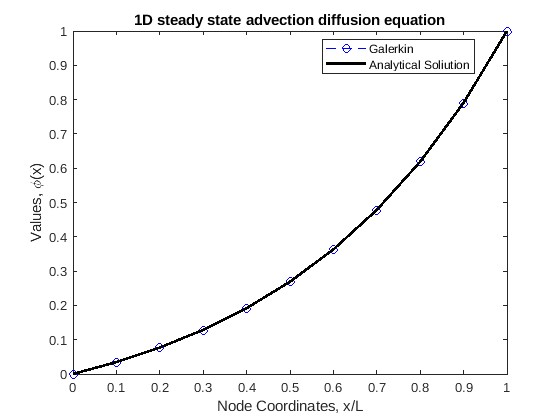
\includegraphics[width=\textwidth]{pe01_no_source.jpg}
	\caption{At Pe = 0.1, L = 1, number of elements = 10, (0, 1) Dirichlet BCs}
	\label{fig-gal-1}
    \end{subfigure}
    \hfill
    \begin{subfigure}[!h]{0.45\textwidth}
	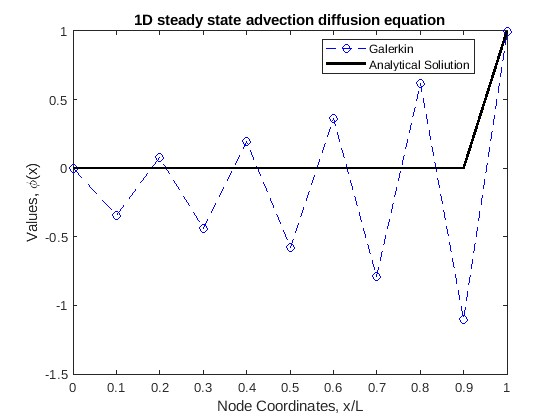
\includegraphics[width=\textwidth]{pe10_no_source.jpg}
	\caption{At Pe = 10, L = 1, number of elements = 10, (0, 1) Dirichlet BCs}
	\label{fig-gal-2}
    \end{subfigure}
    \caption{Galerkin Approximation solution}
\end{figure}
Spurious oscillations in the Galerkin approximation of the advection diffusion reaction equation occurs primarily in advection dominated regimes. The standard Galerkin approximation struggles to resolve the layers in advection dominated regions ($a\ >>\ k $), which causes steep gradients and non-physical oscillations. There are several ways to mitigate these oscillations. 3 are presented in the following sections: Petrov-Galerkin (PG), Stream-Upwind Petrov-Galerkin (SUPG), and Positivity Preserving Variational method (PPV). Compared to PG and SUPG methods, PPV is used to preserve the non-linear positivity condition, making sure discontinuity in the solution are captured and corrected.
\subsection{Petrov-Galerkin Method}
The Galerkin method introduces several problems i.e., sharp gradients and spurious oscillations, in advection dominated problems. These problems or defeciencies can be cured in two ways: one, adding a diffusion term to balance the numerical diffusion introduced by the Galerkin approximation, and two, an upwind approximation of the convective term of the Galerkin solution. Early solutions to the problems in Galerkin method were solved using these two philosophies; however both methodologies are actually equivalent, in that an upwind approximation induces numerical diffusion.\\
The finite element method approximates the advection term with a second order central difference method. Numerical diffusion, however can be introduced by replacing tthe central differencing method by a first-order upwind method, for a $>$ 0:
\begin{equation}
       \begin{aligned}
	    u_x(x_j) \approx \frac{u_j - u_{j - 1}}{h}\\
	    a \frac{u_j u_{j - 1}}{h} - k \frac{u_{j + 1} - 2u_j + u_{j-1}}{h^2} = 0
       \end{aligned}
\end{equation}
Using Taylor expansion for the advection term, an added diffusion of magnitude $\frac{ah}{2}$ is introduced by the upwind approximation. However this upwind treatment of the ADR equation leads to a stable but highly diffusive solution. The Petrov-Galerkin method also utilizes a weighting function that is different than the standard Galerkin method in which $W_a \neq N_a$. For the Petrov-Galerkin method the weighting function becomes
\begin{equation}
       \begin{gathered}
	    W_a = N_a + \alpha W_a^*\\
	    \alpha\ or\ \alpha_{opt} = coth|Pe| - \frac{1}{|Pe|}
       \end{gathered}
\end{equation}
This value of $\alpha$ is chosen to give the exact nodal values for all values of Pe. But, it can be observed from Figure \ref{pe5_no_source} that the solution is over diffusive and deviates from the analytical solution of the governing equation.

\begin{figure}[!h]
\centering
 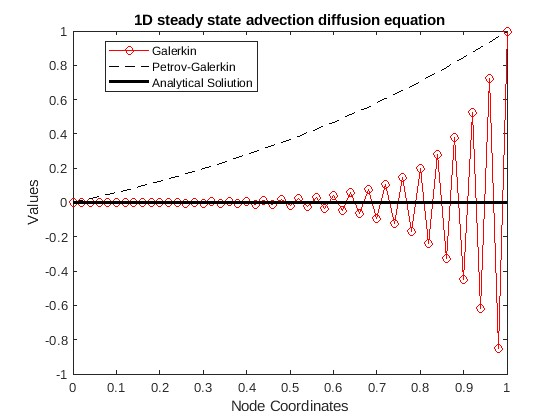
\includegraphics[width=0.7\textwidth]{pe5_pg_no_source.jpg}
\caption{For Pe = 5 with no source}
 \label{pe5_no_source}
\end{figure}   

\subsubsection{Implementation}
\begin{lstlisting}[frame=single, numbers=left, style=Matlab-editor]
function [Klocal_pg, Flocal_pg] = petrovGalerkin(a, mu, h, alpha, nGP, gpts, gwts, elem_dofs, node_coords, soln_full_pg, Klocal, Flocala)
	Klocal = zeros(2, 2);
	Flocal = zeros(2, 1);
    
	n1 = elem_dofs(1);
	n2 = elem_dofs(2);

	u1 = soln_full_pg(n1);
	u2 = soln_full_pg(n2);

	for gp = 1:nGP
		xi = gpts(gp);
		wt = gwts(gp);
		
		N = [0.5 * (1 - xi), 0.5 * (1 + xi)];
		dNdxi = [-0.5, 0.5];
		
		Jac = h / 2;
		
		dNdx = dNdxi / Jac;
		
		% advection
		Klocal = Klocal + (alpha * a * dNdx' * dNdx) * Jac * wt;
		
		% diffusion
		Flocal = Flocal - (alpha * a * dNdx' * du) * Jac * wt;
		end
	Klocal_pg = Klocal_pg + Klocal;
	Flocal_pg = Flocal_pg + Flocal;

end

    
   \end{lstlisting}
This is the subroutine for the Petrov-Galerkin implementation. To implement this correctly, these lines must be added to the pre-processing and the main loop of the main function, respectively.
\begin{lstlisting}[frame=single, numbers=left, style=Matlab-editor]
% at the preprocessing section
alpha = 1 / tanh(Pe) - 1 / (abs(Pe));
\end{lstlisting}
\begin{lstlisting}[frame=single, numbers=left, style=Matlab-editor]
% in the main loop, inside the iteration loop
Kglobal_pg = zeros(totaldof, totaldof);
Fglocal_pg = zeros(totaldof, 1);
% inside the element loop
[Klocal_pg, Flocal_pg] = petrovGalerkin(a, mu, h, alpha, nGP, gpts, gwts, elem_dofs, node_coords, soln_full_pg, Klocal, Flocala);
Kglobal_pg(elem_dofs, elem_dofs) = Kglocal_pg(elem_dofs, elem_dofs) + Klocal;
Fglobal_pg(elem_dofs, 1) = Fglobal_pg(elem_dofs, 1) + Flocal;
\end{lstlisting}
\subsection{Stream-Upwind Petrov-Galerkin Method}
The SUPG method is a stabilization technique used to stabilize the convective term in a consistent manner. This ensures the solution of the differential equation is similar to the solution of the weak form of the governing equation. A standard stabilization technique adds an extra term to the Galerkin weak form, and this term is a function of the residual of the weak form. We know the residual of the ADR equation is  
\begin{equation}
       \begin{gathered}
	   \mathcal{R}(u) = a \cdot \nabla \phi - \nabla \cdot (\nu \nabla \phi) + \sigma \phi - f = \mathcal{L}(u) - f
       \end{gathered}
\end{equation}
Here $\mathcal{L}$ is the differential operator. Now, the standard form of stabilization techniques is 
\begin{equation}
       \begin{gathered}
	   a \cdot \nabla \phi - \nabla \cdot (\nu \nabla \phi) + \sigma \phi + \sum_{e} \int_\Omega \mathcal{P}(w)\tau\mathcal{R}(u) \dd \Omega = f
       \end{gathered}
\end{equation}
where $\tau$ is the stabilization term and $\mathcal{P}(w)$ is the operator applied to the test function. For the SUPG method, the terms are:
    \begin{equation}
           \begin{gathered}
	       \mathcal{P}(w) = a \cdot \nabla w \\
	    \tau = \frac{he}{2a} \left( coth(Pe) - \frac{1}{Pe} \right)
           \end{gathered}
    \end{equation}
\subsubsection{Implementation}
\begin{lstlisting}[frame=single, numbers=left, style=Matlab-editor]
function [Klocal_supg, Flocal_supg] = supg(a, mu, h, alpha, tau, s, nGP, gpts, gwts, elem_dofs, node_coords, soln_full_supg, Klocal, Flocal)
Klocal_supg = zeros(2, 2);
Flocal_supg = zeros(2, 1);

n1 = elem_dofs(1);
n2 = elem_dofs(2);

x1 = node_coords(n1);
x2 = node_coords(n2);

u1 = soln_full_supg(n1);
u2 = soln_full_supg(n2);
u = [u1 u2];

for gp = 1:nGP
	xi = gpts(gp);
	wt = gwts(gp);
	
	N = [0.5 * (1 - xi), 0.5 * (1 + xi)];
	dNdxi = [-0.5, 0.5];
	
	Jac = h / 2;
	
	dNdx = dNdxi / Jac;
	du = dNdx * u';
	uh = N * u';
	x = N * [x1 x2]';
	
	mod_test = a * dNdx';
	
	% stabilization
	Klocal = Klocal + tau * (mod_test * (a * dNdx + s * N) * Jac * wt);
	% force vector
	res = a * du + s * uh - f; % residual
	% Flocal = Flocal + tau * a * dNdx' * f * Jac * wt;
	Flocal = Flocal + tau * (mod_test * f) * Jac * wt;
	Flocal = Flocal - tau * dNdx' * a ^ 2 * du * Jac * wt;
end

Klocal_supg = Klocal_supg + Klocal;
Flocal_supg = Flocal_supg + Flocal;

end
   \end{lstlisting}

\begin{figure}[!h]
\centering
 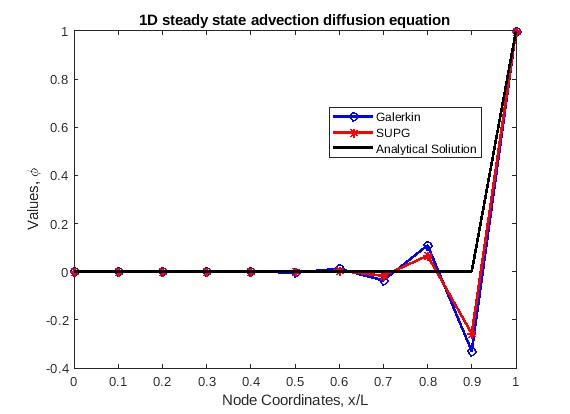
\includegraphics[width=0.7\textwidth]{pe_10_da_10_supg_1_0.jpg}
 \caption{For Pe = 10, Da = 10, (0, 1)}
 \label{pe_10_da_10_1_0_supg}
\end{figure}
This is the subroutine for the SUPG implementation. Similar to the Petrov-Galerkin method, certain variables in the same manner must be initialized before the iteration and the element loop. As seen in Figure \ref{pe_10_da_10_1_0_supg}, the solution to the ADR equation in production regime (s $>$ 1), and even with Pe $>$ 1, the solution is dissipated from its Galerkin approximation solution. The linear stabilization term introduces diffusion and helps stabilize the solution in higher Peclet number cases, but oscillations and sharp gradients still persist. The case in Figure \ref{pe_10_da_10_1_0_supg} is with Pe = 10 and Da = 10, where Da is the Damkohler number and is responsible for the production (s $>$ 0) or destruction (s $<$ 0) regime. The cases from this point onward will include the Da number as part of the problem. The domain for this case constitutes of 10 linear elements, with the left and right nodes being fixed (Dirichlet BC) at $\phi$ = 0 and 1, respectively.
\subsection{Postivity Preserving Variational Method}
To reduce the presence of sharp gradients and oscillations in the solution due to discontinuities, a positivity preserving method is introduced. The PPV method adds a non-linear stabilization term to the weak form of the Galerkin approximation, which is added only when the gradient of the solution is steeper than a certain desired value. It makes sure the solution follows the natural condition and remains within the bounds of the actual solution of the differential equation. Even though SUPG and Petrov-Galerkin methods reduce the oscillations seen in the Galerkin approximation, near discontinuities with sharp gradients overshoots and undershoots still exist. PPV insures the solution follows a natural order -- making sure the solution follows the sign of the neighbour, thus eliminating oscillations.\\
A positivity condition is enforced in the element stiffness matrix i.e.,
   \begin{equation}
       k_{ij} = k_{ji} = max(0, a_{ij}, a_{ji})
 \end{equation}
 where, $a_{ij}$ is an element of the positivity preserving matrix A and $k_{ij}$ is an element of the stiffness matrix. This makes up the sufficient condition for imposing the positivity property to the stiffness matrix. Further, a non linear stabilization term is added to the weak form the Galerkin approximation with SUPG stabilization. Recalling the SUPG stabilized weak form:
 \begin{equation}
    \begin{gathered}
	\int_\Omega w \left( a \cdot \nabla \phi \right) \dd \Omega\ +\ \int_\Omega \nabla w \left( k \nabla \phi \right) \dd \Omega\ +\ \int_\Omega wQ \dd \Omega\ +\ \sum_{e=1}^{n_{el}} \int_\Omega \mathcal{P}(w) \tau \mathcal{R}(\phi) \dd \Omega\ +\\
	\sum_{e=1}^{n_{el}} \int_{\Omega^e} \chi \frac{\abs{\mathcal{R}\left(\phi\right)}}{\abs{\nabla \phi}} k^{add} \frac{\dd w^h}{\dd x} \frac{\dd \phi}{\dd x} \dd \Omega =\ \int_\Omega f N_a \dd \Omega\ +\ \int_\Gamma h N_a \dd \Gamma 
    \label{ppv_eqn}
    \end{gathered}
 \end{equation}
 Here in equation (\ref{ppv_eqn}), the fourth term is the non-linear positivity preserving term. $\mathcal{R(\phi)}$ represents the residual of the advection diffusion reaction equation and $\chi$ is a scaling parameter, which non dimensionalizes $\frac{\abs{\mathcal{R}(\phi)}}{\abs{\nabla \phi}}$. The non-linear term is added to the linear standard weak form, to add the discontinuity (or shock) capturing term. The definitions of $\chi$, $\frac{\abs{\mathcal{R}(\phi)}}{\abs{\nabla \phi}}$, and $k^{add}$ are as follows:
	   \begin{subequations}
	   \begin{align}
	       \chi\ &=\ \frac{2}{\abs{\sigma}h + 2\abs{a}} \label{chi}\\
	       \frac{\abs{\mathcal{R}(\phi)}}{\abs{\nabla \phi}}\ &=\  \frac{\abs{w \left( a \cdot \nabla \phi \right) + w \sigma}}{\abs{\nabla \phi}} \label{res_ratio} \\
	       k^{add} &= max \left\{ \frac{\abs{a - \tau a \sigma + \tau a \abs{\sigma}}h}{2}\ -\ \left( k + \tau a^2 \right)\ +\ \frac{\left( \sigma + \tau \sigma \abs{\sigma} \right)h^2}{6},\ 0\right\} \label{k_add}
	   \end{align}
	   \end{subequations}
\subsubsection{Implementation}
Similar to the Petrov-Galerkin and SUPG implementations, solution $\textit{soln\_full\_ppv}$ and the stiffness matrix, $\textit{Kglobal\_ppv}$ are initialized beforehand. The subroutine for the PPV method goes something like this:
	\begin{lstlisting}[frame=single, numbers=left, style=Matlab-editor]
function [Klocal_ppv, Flocal_ppv] = ppv(a, mu, h, alpha, tau, s, nGP, gpts, gwts, elem_dofs, node_coords, soln_full_ppv, Klocal, Flocal)
Klocal_ppv = zeros(2, 2);
Flocal_ppv = zeros(2, 1);

n1 = elem_dofs(1);
n2 = elem_dofs(2);

x1 = node_coords(n1);
x2 = node_coords(n2);

u1 = soln_full_ppv(n1);
u2 = soln_full_ppv(n2);
u = [u1 u2];

eps = 1e-12;

for gp = 1:nGP
	xi = gpts(gp);
	wt = gwts(gp);
	
	N = [0.5 * (1 - xi), 0.5 * (1 + xi)];
	dNdxi = [-0.5, 0.5];
	
	Jac = h / 2;
	
	dNdx = dNdxi / Jac;
	
	du = dNdx * u';
	uh = N * u';
	
	x = N * [x1 x2]';
	% f = 10.0 * exp(-5 * x) - 4.0 * exp(-x);
	f = 0;
	if (norm(du) < 1e-8)
	    res_ratio = abs((a * dNdx + s * N))/abs((dNdx) + eps);
	    chi = 2 / ((abs(s) * h) + (2 * abs(a)));
	    kadd = max((abs(a - tau*a*s + tau*a*abs(s)) * h / 2) ...
		- (mu + tau*a^2) + (s + tau*s*abs(s)) * h^2 / 6, 0);
	else
	    chi = 0;
	    res_ratio = 0;
	    kadd = 0;
	end
	
	% stabilization
	Klocal = Klocal + chi * res_ratio * kadd * (dNdx' * dNdx) * Jac * wt;
	Flocal = Flocal - res_ratio * chi * kadd * dNdx' * du * Jac * wt;
end

Klocal_ppv = Klocal_ppv + Klocal;
Flocal_ppv = Flocal_ppv + Flocal;

end
	\end{lstlisting}
\begin{figure}[!h]
\centering
 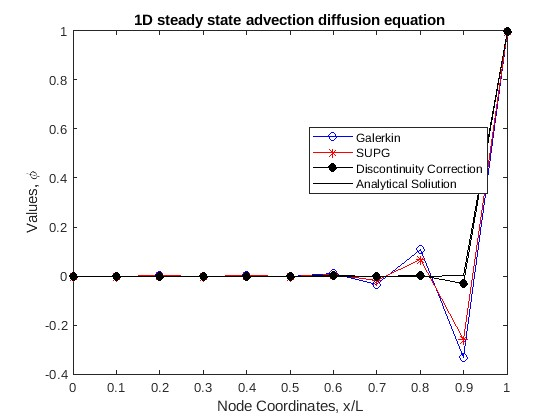
\includegraphics[width=0.6\textwidth]{pe_10_da_10_ppv_0_1.jpg}
 \caption{For Pe = 10, Da = 10 (0, 1) for 10 elements}
 \label{pe_10_da_10_ppv_0_1}
\end{figure}
An error checking condition, that checks for sharp gradients (i.e., norm) is added to the function. This ensures positivity is imparted to the solution, only when discontinuities are observed in the solution. As can be seen in figure \ref{pe_10_da_10_ppv_0_1} as compared to SUPG and Galerkin methods, the solution is more natural i.e., more closely aligned with analytical solution, with little to no oscillations. The domain and initial conditions for this case is the same as that of figure \ref{pe_10_da_10_1_0_supg}.
\section{1D Euler Equations}
The Euler equations of gas dynamics express the conservation of mass, momentum and energy in 3 dimensions, in a compressible, invscid, and non-conducting fluid. The mass conservation equation in Newtonian mechanics, is the law of mass conservation for a varying material $V_t$ occupied by a fluid. The differential form of the mass conversation equation or the continuity equation is
\begin{subequations}
   \begin{gather}
       \frac{\partial \rho}{\partial t} + \rho  \nabla \cdot v = 0 \label{mass_eqn}\\
       \frac{\partial \rho v}{\partial t} + \nabla \cdot \left( \rho v \otimes v + p \textbf{I}\right)v = p \textbf{b} \label{mom_eqn}\\
       \frac{\partial \rho E}{\partial t} + \nabla \cdot \left( \left( \rho E + p \right)  \right) = v \cdot \rho \textbf{b} \label{en-eqn}
   \end{gather}
\end{subequations}
Here $\rho$ is the fluid density and $\rho v$ is the momentum of the fluid. P is the control volume pressure and $\rho E$ is the total energy contained per unit volume. $\rho b$ is the external force per unit volume. In vector forms, the equations can be written as:
\begin{equation}
    \boldsymbol{U_t} + \frac{\partial \boldsymbol{F_1}}{\partial x} + \frac {\partial \boldsymbol{F_2}} { \partial x} = \boldsymbol{B}
\end{equation}
where, \textbf{U} is the conservation variables, $\boldsymbol{F_i}$ are the flux vectors and \textbf{B} is a source term. For 1D Euler equations, the source term and the second flux vector are absent. The terms are defined as follows for one dimensional cases:
\begin{equation}
    \boldsymbol{U} = \left(   \begin{matrix}
			\rho \\
			\rho v \\
			\rho E
		   \end{matrix} \right) \hfill 
    \boldsymbol{F} = \left(   \begin{matrix}
			\rho v_1\\
			\rho v + p \\
			\left( \rho E + p \right) v
		    \end{matrix} \right) \hfill \text{and } p = \left( \gamma - 1 \right) \left[ E - \frac{1}{2} v^2 \right]
    \label{euler-vec}
\end{equation}
The flux jacobian is defined as 
\begin{equation}
    A(U) = F'(U) = \frac {\partial F} { \partial U}
    \label{flux-jac}
\end{equation}
Defining the flux vector in terms of conservative variables makes it easier to understand the flux jacobian matrix.
\begin{equation}
    F(U) =  \left[   \begin{matrix}
		U_2 \\
		\frac{1}{2} \left( 3 - \gamma \right)\frac{U_2^2}{U_1} + \left( \gamma - 1 \right)U_3 \\
		\gamma \frac{U_2 U_3}{U_1} - \frac{1}{2}\left( \gamma - 1 \right)\frac{U_2^2}{U_1^2}
       \end{matrix} \right]
       \label{flux-cons}
\end{equation}
Thus, from equation \ref{flux-jac} and \ref{flux-cons} we get
\begin{equation}
    A(U) = \left[
       \begin{matrix}
	    0 & 1 & 0 \\
	    -\frac{1}{2}\left( \gamma - 3 \right)\left( \frac{U_2}{U_1} \right)^2 & \left( 3 - \gamma \right)\frac{U_2}{U_1} & \gamma - 1 \\
	    -\gamma \frac{U_2 U_3}{U_1^2} & \gamma \frac{U_3}{U_1} - \frac{3}{2}\left( \gamma - 1 \right)\left( \frac{U_2}{U_1} \right)^2 & \gamma \frac{U_2}{U_1}\\
	    
       \end{matrix}
    \right]
    \label{flux-jac-cons}
\end{equation}
Defining the total specific enthalpy H as $H = (E\ +\ p)/\rho$
\begin{equation}
    A(U) = \left[
       \begin{matrix}
	    0 & 1 & 0 \\
	    -\frac{1}{2}\left( \gamma - 3 \right)\left( u\right)^2 & \left( 3 - \gamma \right) u & \gamma - 1 \\
	    u \left[ \frac{1}{2} \left( \gamma - 1 \right)u^2 - H \right] & H - \left( \gamma - 1 \right)u^2 & \gamma u\\
	    
       \end{matrix}
    \right]
    \label{flux-jac-con-mat}
\end{equation}
The Euler equations for gas dynamics is a hyperbolic, non-linear, partial differential equation. To solve it computationally efficiently, it must be first linearized and a solving scheme should be used. For the purpose of the examples, two schemes -- Taylor-Galerkin and Backward Euler method -- are used. 
\subsection{Taylor-Galerkin scheme}
The linear form of the hyperbolic Euler partial differential equations is
\begin{equation}
    \frac {\partial U} { \partial t} + A(U)\frac {\partial U} { \partial x} = 0
    \label{linear-euler}
\end{equation}
Using a Taylor series expansion in time $t\ =\ t^n$, the terms in the equation become
\begin{equation}
\begin{aligned}
    U^{n+1} = U^n + \Delta t \frac {\partial U} { \partial t}\bigg|^n + \frac{\Delta t^2}{2} \frac {\partial^2 u} { \partial t^2}\bigg|^n 
    \label{Un_1eq}
\end{aligned}
\end{equation}
But from equation \ref{linear-euler}, we know, 
\begin{equation}
\begin{gathered}
	\frac {\partial u} { \partial t}\bigg|^n = - A(u)\frac {\partial u} { \partial x}\bigg|^n = - \frac {\partial F} { \partial x}\bigg|^n \\
	\frac {\partial^2 u } { \partial t^2}\bigg|^n = - \frac {\partial } { \partial x} \left( A \frac {\partial u} { \partial t} \right)\bigg|^n = \frac {\partial } { \partial x} \left( A \frac {\partial F} { \partial x} \right)\bigg|^n = \frac {\partial } { \partial x} \left( A^2 \frac {\partial u} { \partial x} \right)\bigg|^n   
	\label{tg-1dudt}
\end{gathered}   
\end{equation}
Then equation \ref{Un_1eq} becomes
\begin{equation}
    \Delta U = - \Delta t \frac {\partial F(U)}{ \partial x} + \frac{\Delta t^2}{2} \frac {\partial } { \partial x} \left( A^2(U) \frac {\partial U} { \partial x} \right) 
\label{tg-var-eq}
\end{equation}
where, $\Delta U$ = $U^{n+1} - U^n$. Now, applying Galerkin approximation as before, i.e., $w = N_a$ and $U = wU$, $w$ is a weighting function and $N_a$ is a basis function. From equation \ref{tg-var-eq},
\begin{equation}
    \frac{1}{\Delta t}M \int \Delta U = - \int F(U) \frac {\partial N_a} { \partial x} \dd x + \Delta t \int A^2(U) \frac {\partial N_a} { \partial x} \frac {\partial N_a} { \partial x} \dd x  \label{tg-var-main}
\end{equation}
Equation \ref{tg-var-main} is the final varitional formulation of the 1D Euler equations using Taylor-Galerkin scheme. The mass matrix $M = \int N_a N_a $ can either be a lumped or a consistent mass matrix. The solution will be second order accurate. The Taylor expansed can be increased in order to find solutions of higher order accuracy.
\subsubsection{Implementation}
For the MATLAB implementation, Sod's shock tube problem was chosen. A domain of with 100 elements was chosen. Sod's shock problem has an initial condition which also acts as the Dirichlet boundary conditions for this problem. The initial conditions are:
\begin{equation}
    x < 0.5 \begin{cases}
    	\rho = 1.0 \\
	u = 0.0 \\
	p = 1.0
	\end{cases} \text{and } x > 0.5 \begin{cases}
    	\rho = 0.125 \\
	u = 0.0\\
	p = 0.1
    \end{cases} 
    \label{init-condn-1d}
\end{equation}
Here the final time $t$ is 0.2 seconds, with $\Delta t = 0.001$. At t = 0, the diaphragm is removed and the resulting flow is characterized. 
\begin{lstlisting}[frame=single, numbers=left, style=Matlab-editor]
close all;
clear; clc;

%% parameters
gamma = 1.4;
x_left = 0.0;
x_right = 1.0;
x_interface = 0.5;

n_elements = 100;
dx = (x_right - x_left) / n_elements;
n_nodes = n_elements + 1;

nGP = 2;
t_final = 0.2;

rho_L = 1.0; u_L = 0.0; p_L = 1.0;
rho_R = 0.125; u_R = 0.0; p_R = 0.1;

x = linspace(x_left, x_right, n_nodes);
U = zeros(3, n_nodes);
U_old = U;

% initial conditions
for i = 1:n_nodes
    if x(i) <= x_interface
	    rho = rho_L; u_gp = u_L; p = p_L;
    else
	    rho = rho_R; u_gp = u_R; p = p_R;
    end
    
    e = p / ((gamma - 1) * rho) + 0.5 * u_gp ^ 2;
    U(:, i) = [rho; rho * u_gp; rho * e];
end

U_L = U(:, 1); U_R = U(:, end);

% mass matrix
M_global = zeros(3 * n_nodes, 3 * n_nodes);

for elem = 1:n_elements
    [gpts, gwts] = get_Gausspoints_1D(nGP);
    M_elem = zeros(6, 6);
    
    Jac_elem = dx / 2;
    
    node1 = elem;
    node2 = elem + 1;
    dof1 = (node1 - 1) * 3 + (1:3);
    dof2 = (node2 - 1) * 3 + (1:3);
    global_dofs = [dof1, dof2];
    
    for gp = 1:nGP
	xi = gpts(gp);
	w = gwts(gp);
	N = [0.5 * (1 - xi), 0.5 * (1 + xi)];
	dN_dxi = [-0.5, 0.5];
	dN_dx = dN_dxi / Jac_elem;
	% assembly
	for i = 1:2
	    i_dofs = (i - 1) * 3 + (1:3);
	    for j = 1:2
		j_dofs = (j - 1) * 3 + (1:3);
		M_ij = N(i) * N(j) * eye(3) * Jac_elem * w;
		M_elem(i_dofs, j_dofs) = M_elem(i_dofs, j_dofs) + M_ij;
	    end
	end
    end
    
    M_global(global_dofs, global_dofs) = M_global(global_dofs, global_dofs) + M_elem;
end

M_lumped = diag(sum(M_global, 2));

% time stepping
t = 0.0;
dt = 0.001;
step = 0;

while t < t_final
    if t + dt > t_final
	dt = t_final - t;
    end
    RHS = zeros(3 * n_nodes, 1);
    for elem = 1:n_elements
	UL = U(:, elem);
	UR = U(:, elem + 1);
	[gpts, gwts] = get_Gausspoints_1D(nGP);
	
	for gp = 1:nGP
	    xi = gpts(gp);
	    wt = gwts(gp);
	    
	    N = [0.5 * (1 - xi), 0.5 * (1 + xi)];
	    dN_dxi = [-0.5, 0.5];
	    Jac_elem = dx / 2;
	    dN_dx = dN_dxi / Jac_elem;
	    u_gp = N(1) * UL + N(2) * UR;
	    
	    [F, A] = calculate_flux_jacobian(u_gp, gamma);
	    % flux
	    flux_term = (F * dN_dx) * Jac_elem * wt;
	    dofs_1 = 3 * (elem - 1) + 1:3 * elem;
	    dofs_2 = 3 * elem + 1:3 * (elem + 1);
	    RHS(dofs_1) = RHS(dofs_1) + flux_term(:, 1);
	    RHS(dofs_2) = RHS(dofs_2) + flux_term(:, 2);
	    % second term
	    ux = [UL, UR] * dN_dx';
	    visc = (A ^ 2) * ux;
	    visc_term = 0.5 * dt * (visc * dN_dx) * Jac_elem * wt;
	    RHS(dofs_1) = RHS(dofs_1) - visc_term(:, 1);
	    RHS(dofs_2) = RHS(dofs_2) - visc_term(:, 2);
	end
    end
    
    delta_U = M_lumped \ RHS;
    U = U + dt * reshape(delta_U, 3, n_nodes);
    U(:, 1) = U_L; U(:, end) = U_R;
    
    if any(~isfinite(U(:)))
	fprintf('NaN/Inf detected at step %d, time %.6f\n', step, t);
	break;
    end
    
    % time update
    t = t + dt;
    step = step + 1;
    fprintf('Step %d: Time = %.4f, dt = %.6f\n', step, t, dt);
end

plot_results(x, U, gamma);

\end{lstlisting}
The subroutines $calculate\_flux\_jacobian$ and $plot\_results$ are as follows:
\begin{lstlisting}[frame=single, numbers=left, style=Matlab-editor]
function [F, A] = calculate_flux_jacobian(U, gamma)
    F = zeros(3, 1);
    A = zeros(3, 3);

    q1 = max(U(1, 1), 1e-10); % rho
    q2 = U(2, 1); % momentum ,rho u
    q3 = U(3, 1); % energy, rho e

    u = q2 / q1;
    p = (gamma - 1) * (q3 - 0.5 * q2 * u);
    H = (q3 + p) / q1;

    F = [q2; q2 * u + p; (q3 + p) * u];
    A = [0, 1, 0; ...
	    0.5 * (gamma - 3) * u ^ 2, (3 - gamma) * u, gamma - 1; ...
	    u * (0.5 * (gamma - 1) * u ^ 2 - H), H - (gamma - 1) * u ^ 2, gamma * u];
end

%% Plot results
function plot_results(x, U, gamma)
    rho = U(1, :);
    u = U(2, :) ./ rho;
    E = U(3, :);
    p = (gamma - 1) * (E - 0.5 * rho .* u .^ 2);

    f1 = figure();
    f2 = figure();
    f3 = figure();
    f4 = figure();

    figure(f1);
    % subplot(2, 2, 1);
    plot(x, rho, 'k-', 'LineWidth', 2);
    title('Density');
    xlabel('x'); ylabel('\rho');
    grid on; ylim([0, 1.2]);

    figure(f2);
    % subplot(2, 2, 2);
    plot(x, u, 'k-', 'LineWidth', 2);
    title('Velocity');
    xlabel('x'); ylabel('u');
    grid on;

    figure(f3);
    % subplot(2, 2, 3);
    plot(x, p, 'k-', 'LineWidth', 2);
    title('Pressure');
    xlabel('x'); ylabel('p');
    grid on; ylim([0, 1.2]);

    figure(f4);
    % subplot(2, 2, 4);
    plot(x, E, 'k-', 'LineWidth', 2);
    title('Total Energy');
    xlabel('x'); ylabel('E');
    grid on;

    % sgtitle('Riemann Shock Tube Solution (Taylor-Galerkin FEM)');
end
\end{lstlisting}
For t = 0.2s the following plot is observed. From the plot, oscillations can be seen present. Thus a stabilization method like SUPG is added to smooth the solution further.
\begin{figure}[!h]
    \captionsetup[subfigure]{justification=centering}
    \centering
    \begin{subfigure}[!h]{0.45\textwidth}
	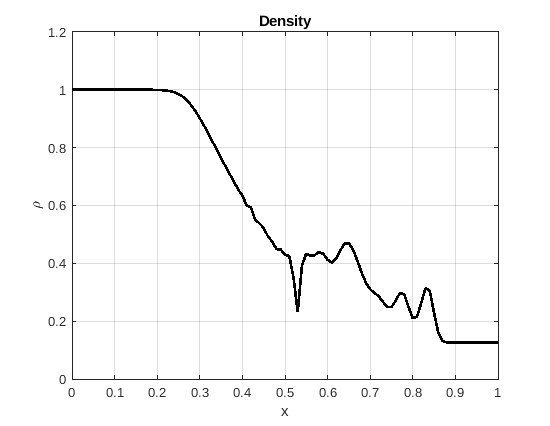
\includegraphics[width=\textwidth]{1d_euler_rho_tg.jpg}
	\caption{Density plot against the length of the domain for t = 0.2s and 100 elements}
	\label{fig-rho-tg}
    \end{subfigure}
    \hfill
    \begin{subfigure}[!h]{0.45\textwidth}
	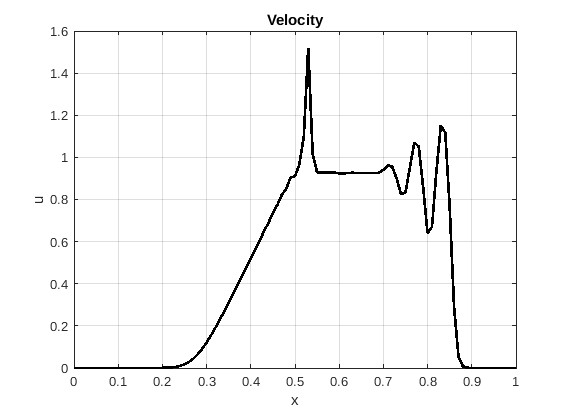
\includegraphics[width=\textwidth]{1d_euler_vel_tg.jpg}
	\caption{Veloctiy plot against the length of the domain for t = 0.2s and 100 elements}
	\label{fig-vel-tg}
    \end{subfigure}
    \begin{subfigure}[!h]{0.45\textwidth}
	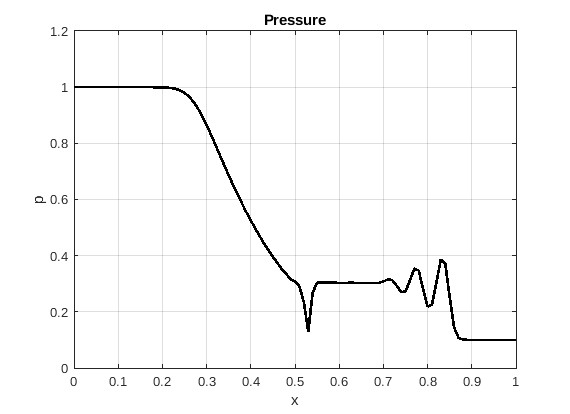
\includegraphics[width=\textwidth]{1d_euler_pres_tg.jpg}
	\caption{Pressure plot against the length of the domain for t = 0.2s and 100 elements}
	\label{fig-pres-tg}
    \end{subfigure}
    \hfill
    \begin{subfigure}[!h]{0.45\textwidth}
	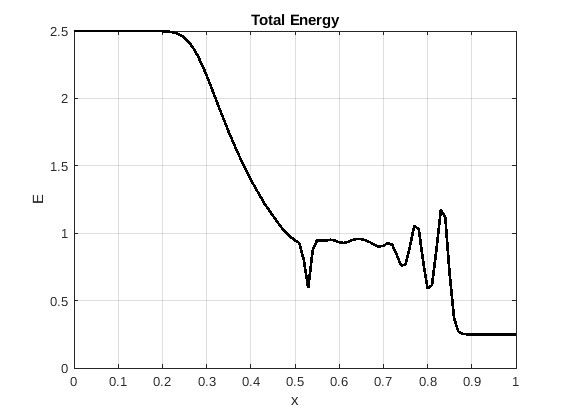
\includegraphics[width=\textwidth]{1d_euler_energy_tg.jpg}
	\caption{Total Energy plot against the length of the domain for t = 0.2s and 100 elements}
	\label{fig-ene-tg}
    \end{subfigure}
    \caption{Taylor-Galerkin scheme for the 1D Euler equations}
\end{figure}
\subsection{Backward Euler scheme}
The backward Euler scheme is an ODE solving technique that utilizes backward differencing, hence backward Euler method, and shifts the solution forward by one time step. Simply put,
\begin{equation}
    \begin{gathered}
	\frac{\dd y}{\dd t} = f \left( t_n, y_n \right) \\
	\frac{y^{n+1} - y^n}{\Delta t} = f \left( t_n, y_n \right) 
    \end{gathered}
    \label{bem}
\end{equation}
Applying it to the 1D Euler equations, we get,
\begin{equation}
    \begin{gathered}
	\frac {U^{n+1} - U^n} {\Delta t} + A(U^n) \frac {\partial U^{n+1}} { \partial x} = 0\\
	\label{bem-1}
    \end{gathered}
\end{equation}
Using Galerkin approximation for equation \ref{bem-1}
\begin{equation}
    \begin{gathered}
	\frac{1}{\Delta t} \int N_a \dd x\ U^{n+1} - \int N_a \dd x\ U^n = - A(U^n) \int N_a  \frac {\partial N_b} { \partial x} \dd x\ U^{n+1} \\
    \end{gathered}
\end{equation}
Rearranging, 
\begin{equation}
    \begin{gathered}
	\left( \int N_a + \Delta t N_a A(U^n) \frac {\partial N_b} { \partial x} \dd x \right) U^{n+1} =  \int N_a \dd x\ U^n \\ 
	\left( \frac{1}{\Delta t} M + K_{stiffness} \right) U^{n+1} = \left( \frac{1}{\Delta t} M \right) U^n  
    \end{gathered}
\end{equation}
\end{document}
